% !TEX root = main.tex

\www{
%After having outlined the preliminaries and the mining model in Sections~\ref{sec:preliminaries} and \ref{sec:pca},
We now outline the core algorithm of AMIE and its implementation.
%Again, we follow the explications in \cite{amie}.
We follow the explications in \cite{amie} and extend them with further explanations and details.
}

\www{
%- - - - - - - - - - - - - - - - - - - - - - - - - - - - - -
\subsection{Algorithm}
\label{subsec:algorithm}
\comment{R2}{Similarly, the Algorithm 2 is not very accurate. It would be clearer if "distinct" is added on line 15: "for all distinct x $\in$ SELECT ?x FROM K WHERE q do." (In contrast, the DISTINCT in the query on the top of Page 11 is redundant).}

\comment{R3}{Here are some of my criticisms, which apply to Section 5 on AMIE - your previous work:
1.Algorithm 1 is too high level and as such it leaves too much unexpressed (e.g. "execute in parallel", "is not pruned for output").
2.      SQL and SPARQL are presented at page 11 only to say that they are discarded for a custom implementation.
3.      The "vanilla in-memory database" implementation is too informally described (e.g.: each "index is a map from the first item to a map from the second item to a set of the third item": a more formal description and a figure, please!
}

\paragraph{Goal} Our goal is to mine rules of the form defined in Section~\ref{sec:preliminaries}.
One of the main problems of any mining approach is to find an efficient way to explore the search space. The naive algorithm of enumerating all possible rules is infeasible for large KBs.
Hence, we explore the search space by iteratively extending rules by \emph{mining operators}.
}

\www{
\paragraph{Mining Operators}
We see a rule as a sequence of atoms. The first atom is the head atom and the others are the body atoms. In the process of traversing the search space, we can extend a rule by using one of the following operators:
\begin{enumerate}
\item \textbf{Add Dangling Atom ($\mathcal{O}_D$})\\
This operator adds a new atom to a rule. The new atom uses a fresh variable for one of its two arguments. The other argument is a variable
that is shared with the rule, i.e., it occurs in some other atom of the rule.
\item \textbf{Add Instantiated Atom ($\mathcal{O}_I$})\\
This operator adds a new atom to a rule that uses an entity for one argument and shares the other argument (variable or entity) with the rule.
\item \textbf{Add Closing Atom ($\mathcal{O}_C$})\\
This operator adds a new atom to a rule so that both of its arguments are shared with the rule.
\end{enumerate}
By repeated application of these operators, we can generate the entire space of rules as defined in Section~\ref{sec:preliminaries}.
The operators generate even more rules than those that we are interested in, because they also produce rules that are not closed.
An alternative set of operators could consist of $\mathcal{O}_D$ and an operator for instantiation.
But these operators would not be monotonic, in the sense that an atom generated by one operator can be modified in the next step by the other operator.
Therefore, we chose the above 3 operators as a canonic set.
}


\paragraph{Algorithm} \label{algo}
Algorithm~\ref{rm} sketches our approach to mine rules. The algorithm maintains a queue of rules, 
which initially contains all possible head atoms, that is,
all rules of size 1.
The algorithm iteratively dequeues a rule from the queue. If the rule 
meets certain criteria (Lines 6 and 7), then it is output.
% \comment{Chris}{its quality is evaluated in terms of (PCA) confidence and if it passes the corresponding threshold} \comment{Luis: }{We threshold on PCA confidence
%  only for AMIE+}\comment{Chris}{so, are we going to output a rule with confidence 0\%?},
Then, if the rule does not exceed the maximum number of atoms $l$ (Line 11), 
the algorithm applies all mining operators to the rule (Lines 12 to 19). This results in more rules which are added to 
the queue if they pass the head coverage threshold $\theta$ (Line 14) and they are not duplicates (Line 14).
This process is repeated until the queue is empty. 
To speed up the process, our implementation parallelizes Algorithm~\ref{rm}, that is, the main loop (Lines 4 to 21) runs
in multiple threads. 
This achieved by synchronizing the access to the centralized queue from which the threads dequeue and enqueue.
% We do not feed predictions of the rules back into the KB. All measures (such as confidence and support) 
% are always computed on the original KB.


% \comment{Chris}{about the figure: shouldn't there be a line stating that the rule is evaluated somehow?}
% Fabian: We discussed this and agreed to leave it as it is until the need arises.

\begin{algorithm}
\caption{Rule Mining}
\label{rm}
\begin{algorithmic}[1]
\Function{AMIE}{KB $\mathcal{K}$, $\theta$, $minConf$, $l$}
    \State $q = [r_1(x,y), r_2(x,y) \dots r_m(x,y)] $
    \State $out = \langle \rangle$
	\While{$\neg q$\emph{.isEmpty}()}
	  \State $r = q.$\emph{dequeue}()
	  \If{$AcceptedForOutput(r, out, minConf)$}
	    \If{$r \notin out$}
	      \State $out.$\emph{add}$(r)$
	    \EndIf
	  \EndIf
	  \If{$length(r) < l$}
	    \ForAll{operators $o$}
	      \ForAll{rules $r' \in o(r)$}
		    \If{$hc(r') \ge \theta$}
		      \If{$r' \notin q$}
			\State $q.$\emph{enqueue}$(r')$
		      \EndIf
		    \EndIf
		  \EndFor
	    \EndFor
	  \EndIf  
	\EndWhile
    \State \Return $out$
\EndFunction
\end{algorithmic}
\end{algorithm}
\ \\[-1cm]
\begin{algorithm}
\caption{Routine to decide to output a rule}
\label{pfo}
\begin{algorithmic}[1]
\Function{AcceptedForOutput}{rule $r$, $out$, $minConf$}
    \If{$r$ is not closed $\vee\; pcaconf(r) < minConf$}
      \State \Return $false$
    \EndIf 
    \State $parents = parentsOfRule(r, out)$
    \ForAll{$r_p \in parents$}
      \If{$pcaConf(r) < pcaconf(r_p)$}
	\State \Return $false$
      \EndIf
    \EndFor
    \State \Return $true$
\EndFunction
\end{algorithmic}
\end{algorithm}

\subsection{Stages of Rule Mining}
\subsubsection{Output a Rule}  
\label{subsubsec:whenToOutput}
Algorithm~\ref{pfo} describes the routine to decide if a rule should be output or 
not once it has been dequeued. If the rule is not closed (See Section~\ref{subsec:rules}) or 
its PCA confidence is below the given confidence threshold, the algorithm discards it for output. 
Recall that AMIE is conceived to mine rules that can predict concrete facts, thus non-closed rules are
seen as intermediate steps. Moreover, the PCA confidence is only defined for closed rules.
It is important to remark, that the confidence threshold is enforced 
very late in the rule mining process, i.e., right before reporting the rule. 
This occurs because confidence is not monotonic, that is, the addition of atoms to a rule
can both increase or decrease its confidence. This means that confidence is not suitable for accurate
pruning. Enforcing the confidence threshold at the end also implies that
the runtime of AMIE is not affected by the magnitude of this value. For this reason, 
the confidence threshold is an optional argument for AMIE. If omitted, the system assumes a value of 0. 

If the rule is closed and confident enough, Algorithm~\ref{pfo} then applies a \emph{skyline technique} (Lines 5 to 10)
to reduce the output. If a rule $B_1 \wedge ... \wedge B_n \wedge B_{n+1} \Rightarrow H$ does not have larger confidence
than its parent rule $B_1 \wedge ... \wedge B_n \Rightarrow H$, then we do not output the longer rule.
Since support and head coverage are monotonic metrics, we know that the child rule will never have a higher score than its parent rule. 
If the child rule has also lower confidence, then its quality is worse in all aspects and there is 
no reason to include it in the output.
In addition, notice that a rule can have multiple parents, for instance, the rule $actedIn(x,y) \wedge directedIn(x,y) \Rightarrow created(x,y)$
can be derived by applying a closing-atom operator $\mathcal{O}_C$ to either $actedIn(x,y) \Rightarrow created(x,y)$ or
$directedIn(x,y) \Rightarrow created(x,y)$. AMIE
finds all the potential parents of a rule (Line 5) and applies the skyline technique to each of them (Lines 6 to 10), i.e., the child
rule must have higher confidence than all its parents to be accepted for output.
We emphasize that the skyline technique is only applied to prune the output. 
Since confidence can increase with the addition of atoms, we should still use the longer rule 
for further refinement.

\paragraph{Count Queries for Confidence} By the time a rule is dequeued, AMIE already know its support. 
Recall from Section~\ref{subsubsec:pcaConf} that the PCA confidence is defined according to the formula:
\[
\begin{small}
conf_{pca}(\vec{B} \Rightarrow r(x,y)) := \frac{supp(\vec{B} \Rightarrow r(x,y))}{\#(x,y): \exists z_1,...,z_m,y': \vec{B} \wedge r(x,y')}
\end{small}
\]
That is, to compute the confidence of a rule AMIE must fire a \emph{count query} to estimate the denominator
of the confidence formula. For the PCA confidence, such queries have the form: \\

\noindent{SELECT COUNT($H'$) WHERE $H \wedge B_1 \wedge ... \wedge B_n$} \\

\noindent where $H$ is the head atom, $B_1, \dots, B_n$ are the body atoms and $H'= r'(x,y')$ is a variant of the
head atom where the least-functional variable has been replaced by a fresh variable (see Section~\ref{subsubsec:pcaConf}).
We will discuss the implementation of such queries and their relation to SPARQL and SQL queries in Section~\ref{subsec:implementation}. 
For now, we will use the above pseudo-syntax.

\subsubsection{Specialization}
\label{subsubsec:specialization}

The application of the mining operators to a rule (Algorithm~\ref{rm}, Lines 12 to 19), produces multiple new rules. 
All these rules are identical to the original rule, except that they contain
a new atom. In addition, such rules are required to fullfill the head coverage constraint (Line 13). No matter which operator is applied in particular, Algorithm~\ref{rm} needs to choose relations
for the new atoms. Furthermore, the instantiation operator $\mathcal{O_I}$ also allows the choice of an entity in one 
of the arguments of the new atom.
In order to select only relations and entities that will fulfill the head coverage constraint, 
we rely on the KB to answer \emph{count-projection queries}.
These are queries of the form
\indented{SELECT $\bm{x}$, COUNT($H$) \\
WHERE $H \wedge B_1 \wedge ... \wedge B_n$\\
SUCH THAT COUNT($H$)$\geq k$}

\noindent where $H, B_1, ..., B_n$ are atoms and $k$ is a natural number.
$\bm{x}$ is the \emph{selection variable}.
It is a variable that appears in one or more atoms at the position of one of the arguments or at the position of the relation (as it is common in SPARQL~\cite{sparql}). 
Such queries select an entity or relation $x$ such that the result of the query $H \wedge B_1 \wedge ... \wedge B_n$ on the KB contains more than $k$ distinct query answers
for the \emph{group atom} $H$. The group atom corresponds to the head of the rule.
% Fabian: we never said it, so the reader cannot recall
%Recall that the expression COUNT($H$) binds to the support
%of the whole query pattern for each value of the selection variable $?x$.
We defer the implementation of such type of queries to Section~\ref{subsec:implementation}.


\paragraph{Count-Projection Queries} Count-projection queries allow us to select the relationship for the operators 
$\mathcal{O_D}$, $\mathcal{O_I}$, and $\mathcal{O_C}$ in such a way
that the head coverage of the resulting rule is above $\theta$.
This works by firing a projection query of the form
\\ \\
SELECT $\bm{r}$, COUNT($H$)\\
WHERE $H \wedge B_1 \wedge ... \wedge B_{n-1}\; \wedge\; \bm{r}(\bm{X},\bm{Y})$\\
SUCH THAT COUNT($H$)$\geq k$
\\ \\
%\comment{Katja}{HAVING without GROUP BY, see above}
where $k := \theta \times size(H)$ (see Section~\ref{par:headCoverage}) is the translation of the
head coverage threshold into an absolute support threshold. $\bm{X}$ and $\bm{Y}$ are meta-variables that
can be either variables or constants, 
depending on the type of atoms that the operator generates, e.g., when applying the $\mathcal{O}_I$ operator, 
at least one of this meta-variables binds to a constant.
The results for $\bm{r}$ are the relations that, once bound in the query, ensure that the head coverage 
of the rule $B_1 \; \wedge ... \wedge B_{n-1} \;\wedge\; \bm{r}(\bm{X},\bm{Y}) \Rightarrow H$ is greater than $\theta$.
Notice also that for each value of $\bm{r}$, the expression COUNT($H$) gives us the support of the new rule.
For instance, assume Algorithm~\ref{rm} dequeues the following intermediate non-closed rule for further specialization.

\begin{center}
\emph{marriedTo}$(x,z) \Rightarrow $ \emph{livesIn}$(x,y)$
\end{center}

\noindent
The application of the operator $\mathcal{O_D}$ will fire queries of the form:\\ \\
SELECT $\bm{r}$, COUNT($livesIn(x,y)$) \\
WHERE $livesIn(x,y) \; \wedge \; marriedTo(x,z) \wedge \bm{r}(\bm{X}, \bm{Y})$\\
SUCH THAT COUNT($livesIn(x,y)$)$\ge k$\\

\noindent with 
\[
\bm{r}(\bm{X}, \bm{Y}) \in \{\bm{r}(x,w), \bm{r}(z,w), \bm{r}(w,x), \bm{r}(w,z) \}
\]
That is $\bm{r}(\bm{X}, \bm{Y})$ binds to each possible join combination of a new dangling atom,
where $w$ is an arbitrary fresh variable. For intermediate rules, dangling atoms are joined on the non-closed variables; 
$z$ and $y$ in this example.
If the rule is closed, dangling atoms are joined on all the variables appearing in the rule.

In the same fashion, when applying the $\mathcal{O_C}$ operator to our example, the atom $\bm{r}(\bm{X}, \bm{Y})$ 
can take values in $\{ \bm{r}(z,y), \bm{r}(y,z) \}$.
% \\ \\
% SELECT $?r$, COUNT($livesIn(x,y)$)\\
% WHERE $livesIn(x,y) \wedge isMarriedTo(x,z) \wedge\; ?r(z,y)$\\
% SUCH THAT COUNT($livesIn(x,y)$)$>= k$
% \\ \\
%\comment{Katja}{HAVING without GROUP BY, see above}
%is one of the ways to apply the operator $\mathcal{O_C}$.
The method will produce new atoms so that all open variables are closed. In this example, the method produces the minimum number
of specializations required to close the variables $y$ and $z$. If there is only one closed variable, the method will produce atoms between
the open variable and all the other variables. If the rule is already closed, the operator tries with
all possible pairs of variables in the rule.

Finally, the instantiation operator $\mathcal{O_I}$ is implemented in two steps. 
We first apply the operator $\mathcal{O_D}$ to produce a set of intermediate rules 
with a new dangling atom and a new fresh variable.
Then for each rule, we fire a count-projection query on the fresh variable. 
This step provides bindings for one of the arguments of the relation.
For instance, the implementation of the $\mathcal{O_I}$ operator to our example 
rule 
\begin{center}
\emph{marriedTo}$(x,z) \Rightarrow $ \emph{livesIn}$(x,y)$
\end{center}

\noindent will first add all possible dangling atoms to the rule. Let us consider one group of such atoms, e.g., those of the form
$\bm{r}(x,w)$. Then for each
value of $\bm{r}$ that keeps the rule above the head coverage threshold $\theta$, the algorithm tries to find the best bindings for 
$w$. For example, imagine we bind $\bm{r}$ to the relation $citizenOf$. The second step will fire a query of the form:
\\\\
\noindent
SELECT $\bm{w}$, COUNT($livesIn(x,y)$) WHERE \\ 
$livesIn(x,y) \wedge marriedTo(x,z) \wedge citizenOf(x,\bm{w})$ \\
SUCH THAT COUNT($livesIn(x,y)$)$\ge k$\\

\noindent Each binding of $\bm{w}$ forms a new rule that will be enqueued and later evaluated for output.

In the way described above, projection queries allow us to choose the relationships and entities for the operators 
in such a way that the head coverage for the new rules is guaranteed to be above $\theta$.
We discuss how to implement projection queries efficiently in Section~\ref{subsec:implementation}.

\subsubsection{Pruning} 
\label{subsubsec:pruning}
\www{
If executed naively, Algorithm~\ref{rm} will have prohibitively high runtimes.
The instantiation operator $\mathcal{O}_I$, in particular, generates atoms in the order of $|\mathcal{R}| \times |\mathcal{E}|$.
We first observe that we are usually not interested in rules that cover only very few facts of the head relation.
Rules that cover, for example, less than 1\% of the facts of the head relation can safely be assumed to be marginal.
Therefore, we choose $\theta=0.01$ as a lower bound for the head coverage. We observe that head coverage decreases monotonically as we add more atoms.
This allows for safely discarding any rule that trespasses the threshold (lines 11 and 12 in Algorithm~\ref{rm}).
}
Recall from Section~\ref{subsec:statSignificance} that support and head coverage are defined even for rules that are not yet closed, allowing for early pruning.

\subsubsection{Duplicate elimination} 
\label{subsubsec:duplicateElimination}
As mentioned in Section~\ref{subsubsec:whenToOutput} a rule can be derived in multiple ways.
For example, the rule $actedIn(x,y) \wedge directedIn(x,y) \Rightarrow created(x,y)$ can result from the application
of the operator $\mathcal{O}_C$ to both $actedIn(x,y) \Rightarrow created(x,y)$ and $directedIn(x,y) \Rightarrow created(x,y)$.
This implies that the specialization section (Lines 11 to 19) of Algorithm~\ref{rm} can lead to duplicate rules.
For this reason, the AMIE algorithm does a duplicates checking before queueing a rule (Line 14). 
While checking two rules for equality is expensive (it is a graph isomorphism verification task), 
we observe that two rules can only be equal if they have the same head relation, the same number of atoms and
the same head coverage (or support). This reduces drastically the set of rules that have to be checked and therefore
the time invested in this task. 

In addition, Algorithm~\ref{rm} also checks duplicates in the output (Line 7). This particular checking step 
is necessary only in the presence of multithreading. Recall that our algorithm performs a breadth-first-search. 
This means that in a fully sequential execution, rules of size $n-1$ are always queued before rules of size $n$. 
It follows that, by the time we check the duplicates of a rule of size $n$ to enqueue it (Line 14 in Algorithm~\ref{rm}), 
no rule of size $n$ has still been dequeued. In other words, if a rule is the duplicate 
of another rule already derived, the original rule must be in the queue. This property guarantees no duplicates at output time. 
However, this does not hold in a multi-threading environment. To see this, imagine that rules 
$R_n$ and $R'_n$ are both in the queue at timestamp $t_0$ and both can refined into rule $R_{n+1}$
by means of the mining operator $o$. 
Moreover, consider two threads $T_1$ and $T_2$ and the sequence of events depicted in Table~\ref{tab:duplicates}.

\begin{table}
\centering
 \begin{tabular}{c|l|l}
  Timestamp & $T_1$ & $T_2$\\  \hline
  $t_1$ & $R_n = q.dequeue()$	&  \\
  $t_2$ & & $R'_n = q.dequeue()$ \\
  $t_3$ & $R_{n+1} = o(R_n)$  & \\
  $t_4$ & $q.enqueue(R_{n+1})$  & \\
  $t_5$ & $R_{n+1} = q.dequeue()$ & \\
  $t_6$ & & $R_{n+1} = o(R_n)$ \\
  $t_7$ & & $q.enqueue(R_{n+1})$ \\
\end{tabular}
\caption{An execution scenario that could lead to duplicate rules in the output.}\label{tab:duplicates}
\end{table}

In this example, we enqueue the rule $R_{n+1}$ twice, at timestamps $t_4$ and $t_7$. 
Since $T_1$ dequeues $R_{n+1}$ before $T_2$ also finds it, 
we cannot know that the rule was already output before. Since duplicate verification
can be performed very efficiently, we show that the time invested in this additional step does not the 
outweight the benefit of using multiple threads.


\subsection{Implementation} \label{subsec:implementation}

\paragraph{SQL and SPARQL} Count-projection queries are essential for the efficiency of our system. 
Yet, standard database implementations do not provide special support for these types of queries. 
Assuming that the KB $\mathcal{K}$ is stored as a three-columns table, i.e., each fact is a row with three columns 
$\langle s, r, o \rangle$, the count-projection query template in SQL would be: \\ \\
% \indented{SELECT DISTINCT R.$?x$, SUM(R.$N$) FROM (\\
% \hspace*{1ex} SELECT $?x$, COUNT(*) AS N \\
% \hspace*{1ex} FROM $\mathcal{K}$ AS H, $\mathcal{K}$ AS $B_1$, \dots $\mathcal{K}$ AS $B_n$ \\
% \hspace*{1ex} WHERE $H.x_i$ = $B_j.x_m$ AND \dots \\
% \hspace*{1ex} GROUP BY $?x$, $H.x_1$, $H.x_r$, $H.x_2$) AS R \\
% GROUP BY R.$?x$ \\
% HAVING SUM(R.$N$) $>= k$
% }
\noindent{SELECT $\mathcal{C}.\bm{c}$, $COUNT(*)$ FROM $\mathcal{K}$ AS H, \\
(SELECT DISTINCT $\bm{c}$ FROM $\mathcal{K}$) AS $\mathcal{C}$ \\ 
 WHERE $\bm{P}(H)$ AND EXISTS \\
\hspace*{1ex} (SELECT * FROM $\mathcal{K}$ AS $B_1$, $\dots \mathcal{K}$ AS $B_n$ \\
\hspace*{2ex} WHERE $\bm{P'}(H, B_1, \dots B_n)$) \\
GROUP BY $\mathcal{C}.\bm{c}$ HAVING $COUNT(*) >= k$ \\
}

\noindent Here, $B_n$ is the new atom added to the query and $\bm{c} \in \{s, r, o\}$. 
The temporary table $\mathcal{C}$ contains the target values for the new atom, e.g., relations
if $\bm{c} = r$. The function $\bm{P}(H)$ represents the conditions imposed by the head atom, e.g., for a rule
of the form $\vec{B} \Rightarrow livesIn(x, USA)$, $\bm{P}(H)$ is translated into 
$H.r = ``marriedTo"\; \text{AND}\; H.o = ``USA"$. Likewise, the function $\bm{P'}(H, B_1, \dots B_n)$
is replaced by the join conditions between the head and body atoms. 
If we apply this scheme to the addition of a closing atom $\bm{r}(z,y)$ in our example rule
\emph{marriedTo}$(x,z) \Rightarrow $ \emph{livesIn}$(x,y)$, we would generate the query
% \indented{SELECT $R.x_r$, SUM($R.N$) FROM ( \\
%  \hspace*{1ex} SELECT $B_2.x_r$ AS $x_r$, COUNT(*) AS N\\
%  \hspace*{1ex} FROM $\mathcal{K}$ AS H, $\mathcal{K}$ AS $B_1$, $\mathcal{K}$ AS $B_2$\\
%  \hspace*{1ex} WHERE $H.x_1$ = $B_1.x_1$ AND $H.x_2 = B_2.x_2$ \\
%  \hspace*{1ex} AND $B_2.x_1 = B_1.x_2$ AND $H.x_r = ``livesIn"$ \\
%  \hspace*{1ex} AND $B_1.x_r = ``marriedTo"$ \\
%  \hspace*{1ex} GROUP BY $B_2.x_r$, $H.x_1$, $H.x_r$, $H.x_2$) AS R\\
%  GROUP BY $R.x_r$ \\
%  HAVING SUM($R.N$) $>= k$
% }
\\\\
\noindent{SELECT $\mathcal{R}.r$, $COUNT(*)$ FROM $\mathcal{K}$ AS H, \\
(SELECT DISTINCT $r$ FROM $\mathcal{K}$) AS $\mathcal{R}$ WHERE $H.r = ``livesIn"$ AND EXISTS \\
\hspace*{1ex} (SELECT * FROM $\mathcal{K}$ AS $B_1$, $\mathcal{K}$ AS $B_2$, \\
\hspace*{2ex} WHERE $H.s = B_1.s$ AND $H.o = B_2.o$ \\
\hspace*{2ex} AND $B_2.s = B_1.o$ AND $B1.r = ``isMarriedTo"$ \\
\hspace*{2ex} AND $B_2.r = \mathcal{R}.r$) \\
GROUP BY $\mathcal{R}.r$ HAVING $COUNT(*) >= k$ \\ \\
}
\noindent The query stores all possible relations for the new atom in the temporary table $\mathcal{R}$ and
applies a semi-join with the head atom $H$. The semi-join is constrained to those bindings of $\mathcal{R}$ for 
which there exists at least one binding in the rule. The results are then grouped (GROUP BY), aggregated (COUNT(*)) 
and thresholded (HAVING) per binding of the new atom.
Our experience shows that for a KB of a few million facts, such kind of queries 
can easily take several minutes on an off-the-shelf RDBMS.
Hence, efficient SPARQL engines such as RDF-3X \cite{rdf3x} are an alternative option. 
In SPARQL 1.1, the count-projection query template is: \\
% \indented{SELECT $?x$, SUM($?support$) \\
%  WHERE \{ \\
%  \hspace*{2ex} SELECT $?x$, COUNT(*) AS $?support$ \\
%  \hspace*{2ex} WHERE \{ \\
%  \hspace*{4ex} $H.x_1$, $H.x_r$, $H.x_2$ . \\
%  \hspace*{4ex} $B_1.x_1$, $B_1.x_r$, $B_1.x_2$ . \\
%  \hspace*{4ex} \dots \\
%  \hspace*{4ex} $B_n.x_1$, $B_n.x_r$, $B_n.x_2$ . \\
%  \hspace*{2ex} \} \\
%  \hspace*{2ex} GROUP BY $?x, H.x_1$ $H.x_r$ $H.x_2$ \\
%  \} \\
%  GROUP BY $?x$ HAVING SUM($?support$) $ >= k$ \\
% }
\\
\noindent{SELECT $\bm{c}$, SUM($?supp$) WHERE \{ \\
 \hspace*{2ex}  SELECT $\bm{c}$ (COUNT(DISTINCT *) AS $?supp$) \\
 \hspace*{2ex} WHERE \{ \\
 \hspace*{4ex} SELECT $\bm{c}$ COUNT(DISTINCT *) AS $?support$ \\
 \hspace*{4ex} WHERE \{ \\
 \hspace*{6ex} SELECT $\bm{c}$ $?s_H$ $?o_H$ WHERE \{ \\
 \hspace*{6ex} $?s_H$ $r_H$ $?o_H$ . \\
 \hspace*{6ex} $?s_1$ $r_1$ $?o_1$ . \\
 \hspace*{6ex} \dots \\
 \hspace*{6ex} $?s_n$ $?r_n$ $?o_n$ . \\
 \hspace*{6ex} \} GROUP BY $?x, H.x_1$ $H.x_r$ $H.x_2$ \\
 \hspace*{4ex}\} GROUP BY $\bm{c}$ $?s_H$ $?o_H$ \\
 \} GROUP BY $\bm{c}$ HAVING SUM($?supp$) $ >= k$ \\
} \\
% SELECT ?relation (sum(?support) as ?N) WHERE {
% SELECT ?relation (count(DISTINCT *) as ?support) WHERE {
%   SELECT DISTINCT ?relation ?x ?y WHERE {      
%       ?x <http://localhost:3030/kb/livesIn> ?y .
%       ?x <http://localhost:3030/kb/marriedTo> ?z .
%       ?z ?relation ?y .
%   }
% } GROUP BY ?relation ?x ?y
% } GROUP BY ?relation
\noindent where $\bm{c} \in \{ ?s_n, ?r_n, ?o_n \}$ is a variable associated to new atom added to the rule
and the triple pattern $\langle ?s_H \; r_H \; ?o_H \rangle$ corresponds to the head atom. This particular template models the case
where the head atom does not contain constants. If it not the case, e.g., $\vec{B} \Rightarrow livesIn(x, USA)$, 
we simply replace the argument variables $?s_H$ or $?o_H$ by the corresponding constant and remove it from the GROUP BY condition.  
As grouping and aggregate functions have only recently become part of the SPARQL 1.1 standard, 
many existing SPARQL engines do not yet efficiently support the extension. Moreover 
RDF-3X does not support aggregate functions in this way. 
Thus, we would need extensive postprocessing of query results to compute a projection query.
Hence, we resorted to a custom implementation.

\paragraph{In-Memory Database} We have implemented a vanilla in-memory database for semantic KBs.
Our implementation indexes the facts aggressively with one index for each permutation of 
the columns subject, relation, and object, i.e., there are six indexes, namely \texttt{SRO}, \texttt{SOR}, 
\texttt{RSO}, \texttt{ROS}, \texttt{OSR} and \texttt{ORS}. We call them \emph{fact indexes}.
Each fact index consists of a nested hash table, where the keys are the values for the first column and the items
are second-level hash tables. The second-level hash tables map from values of the second column
to sets of values of the third column. 
Figure~\ref{indexes} illustrates the structure of the fact index \texttt{RSO} for a set of four facts.
Fact indexes allow us to check the existence of a triple in constant time.

\begin{figure}
%\hspace*{-5ex}
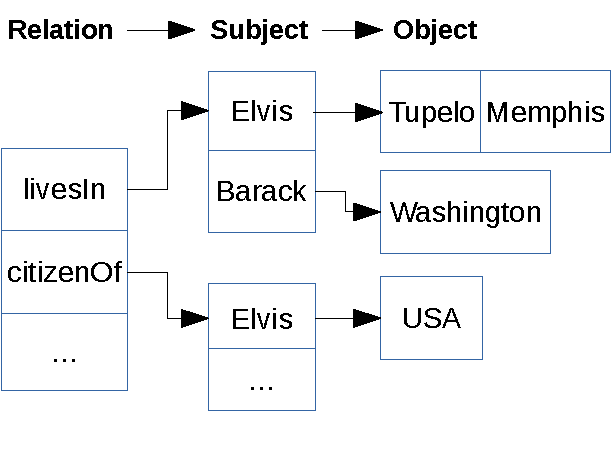
\includegraphics[width=0.5\textwidth]{figures/indexes}\
\caption{Structure of the fact index RSO for a set of four facts}
\label{indexes}
\end{figure}

In addition to the fact indexes, the database relies 
on three \emph{aggregated indexes} \texttt{S}, \texttt{P}, \texttt{O} that store the aggregated number of facts for each
key of the fact indexes. For example, the aggregated index \texttt{P} stores the number of triples for each relation
in the KB, e.g., $\{ livesIn=3, citizenOf=1 \}$ for the fact index depicted in Figure~\ref{indexes}. 
Fact indexes in combination with aggregated indexes can be used to determine the size of atom, i.e., its number of bindings, 
in constant time. For example, the size of the atom $livesIn(x,y)$ can be retrieved by a simple look-up 
in the aggregated index \texttt{P}. In constrast, the size of the atom $livesIn(x, USA)$ requires two 
lookups in the fact index \texttt{ROS}: the first lookup to get the object values of $livesIn$ and the second
to retrieve the list of subjects for the object value $USA$. 

The existence of a query answer can be checked naively by (1) selecting the atom with fewest instantiations using the indexes, 
(2) running through all of its instantiations, (3) instantiating the remaining atoms accordingly and (4)
repeating this process recursively until we find an instantiation of the query that appears in the KB.
Select queries can be implement on top of this procedure by storing the instantiations for the variables
in the projection as we run through them.


\paragraph{Implementation of Count-Projection Queries} Algorithm \ref{algi} shows how we answer count-projection queries.
The algorithm takes as input a selection variable $\bm{x}$, a projection atom $H:=R(\bm{X},\bm{Y})$, remaining atoms $B_1, ... B_n$, 
and a KB $\mathcal{K}$. If the routine is used to find the relations for a new atom in a rule, e.g., $\bm{r}(\bm{Z}, \bm{W})$, then 
$\bm{x} = \bm{r}$. We first check whether $\bm{x}$ appears in the projection atom (Line 3).
If that is the case (Lines 4 to 10), we run through all instantiations of the projection atom, instantiate the query accordingly, and check for existence.
Each existing instantiation increases the counter for the respective value of $?x$. 
If the selection variable does not appear in the projection atom, we iterate through all instantiations of the projection atom.
We instantiate the query accordingly, and fire a SELECT query for $?x$. We increase the counter for each value of $?x$. We report all values whose counter exceeds $k$.



\paragraph{Summary}
The AMIE algorithm iteratively builds more complex rules from simpler rules by the help of three operators.
It takes advantage of monotonic measures to prune the search space efficiently and also takes care of duplicate elimination.
We have identified projection queries as the crucial type of queries for rule mining.
Since standard database systems and standard SPARQL systems provide no specifically tuned support for these queries,
we have implemented a vanilla in-memory database, which has specific support for projection queries.
Our entire implementation is in Java. The code can be downloaded from our Web site\footnote{\url{http://mpi-inf.mpg.de/departments/ontologies/projects/amie}}.

\www{

\begin{algorithm}
\caption{Answering Projection Queries}
\label{algi}
\begin{algorithmic}[1]
\Function{SELECT}{$\bm{x}$, $R(X,Y) \wedge B_1 \wedge ... \wedge B_n$, $k$, $\mathcal{K}$}
    \State $map = \{\}$
    \If {$\bm{x} \in \{R,X,Y\}$}
	  \ForAll{instantiations $r(x,y)$ of $R(X,Y) \in \mathcal{K}$}
	    \State $q=B_1 \wedge ... \wedge B_n$
		\State In $q$, replace $X$ by $x$, $Y$ by $y$
	    \If{exists instantiation $q \in \mathcal{K}$}
		\State $map[x]++$
		\EndIf
	  \EndFor
	\Else
	  \ForAll{instantiations $r(x,y)$ of $R(X,Y) \in \mathcal{K}$}
	    \State $q=B_1 \wedge ... \wedge B_n$
		\State In $q$, replace $R$ by $r$, $X$ by $x$, $Y$ by $y$
	    \ForAll{$x\in${\small{}SELECT $?x$ FROM $\mathcal{K}$ WHERE $q$}}
		  \State $map(x)++$
		\EndFor
	  \EndFor
	\EndIf
	\State \Return $map$
\EndFunction
\end{algorithmic}
\end{algorithm}
\ \\[-1cm]
}